%% ----------------------------------------------------------------
%% Project.tex
%% ---------------------------------------------------------------- 
\documentclass[oneside]{ecsproject}     % Use the Project Style
\graphicspath{{../Figures/}}   % Location of your graphics files
\hypersetup{colorlinks=true}   % Set to false for black/white printing
\usepackage{longtable}         % Tables that span multiple pages
\usepackage{tabularx}          % Full-width tables with flexible columns
%% ----------------------------------------------------------------

\begin{document}
\frontmatter
\pagenumbering{roman}

% =========================
% FRONT TITLE PAGE
% =========================
\begin{titlepage}
\thispagestyle{empty}
\centering

\vspace*{-1.2cm}

% ---- University Logo ----

\includegraphics[width=0.60\textwidth]{figures/tiu.png}\par
\vspace{0.25cm}

% ---- Project Title ----
{\Large\bfseries
EduFeedBack AI: Post-Career Analytics \& Curriculum Refinement\par}

\vspace{0.25cm}

{\normalsize\bfseries 8th Semester Project Report}\\

\vspace{0.2cm}

% ---- Submission ----
{\small submitted to}\par
{\normalsize\bfseries Techno India University, West Bengal}\par

\vspace{0.2cm}

{\small In partial fulfilment of the requirements}\\
{\small for the award of the degree of}\\

\vspace{0.15cm}

{\normalsize\bfseries Bachelor of Technology}\\

\vspace{0.1cm}

{\small in}\\
{\normalsize\bfseries Computer Science \& Engineering}\\

\vspace{0.15cm}

% ---- Students ----
{\small by}\par
\vspace{0.1cm}

\begin{tabular}{c}
\textbf{Khandakar Aryanul Haque (Roll No. 221001001282)}\\
\textbf{Navita Verma (Roll No. 221001001315)}\\
\textbf{Junaid Akhter (Roll No. 221001001316)}\\
\textbf{Ruchita Mishra (Roll No. 221001001324)}\\
\textbf{Aryan Hela (Roll No. 221001001332)}
\end{tabular}

\vspace{0.2cm}

% ---- Supervisor ----
{\small Under the guidance of}\par
{\normalsize\bfseries Dr. Soumi Paul}\par

\vspace{0.35cm}

% ---- Footer ----
{\small Department of Computer Science \& Engineering}\par
{\small\bfseries TECHNO INDIA UNIVERSITY, WEST BENGAL}\par

\vspace{0.1cm}

{\small April 2026}\par

\vfill

{\small © 2026, Techno India University. All rights reserved.}

\end{titlepage}

% =========================
% DEDICATION PAGE
% =========================
% Omitted unless requested, as none was found in the PDF.

% =========================
% AUTHOR DECLARATION
% =========================
\begin{declaration}
We hereby declare that the project report entitled \textbf{``Post-Career Analytics \& Curriculum Refinement''} is an authentic record of our own work carried out at the \textbf{Department of Computer Science and Engineering, Techno India University, West Bengal}, during the \textbf{8th semester of the academic year 2025--2026} under the supervision of \textbf{Dr. Soumi Paul}, Assistant Professor.

We further declare that the matter embodied in this project report has not been submitted by us for the award of any other degree or diploma of this or any other Institute/University. All the information have been
obtained and presented in accordance with academic rules and ethical conduct.
We also declare that, as required by these rules and conduct, we have fully cited and referenced all materials and results that are not original to this work.

\vspace{1.2em}

\noindent
\textbf{Place:} EM-4/1, Sector V, Bidhannagar, Kolkata, West Bengal -- 700091
\par\vspace{0.1cm}
\textbf{Date:} April 2026

\vspace{0.7em}

\noindent
\textbf{Signatures:}

\vspace{0.1em}

\noindent
\begin{center}
\begin{tabular}{p{0.45\textwidth} p{0.45\textwidth}}
\textbf{Signature:} \rule{4.5cm}{0.4pt} &
\textbf{Signature:} \rule{4.5cm}{0.4pt} \\[-0.2em]
\textbf{Name: Khandakar Aryanul Haque} &
\textbf{Name: Navita Verma} \\[-0.2em]
\textbf{Roll No: 221001001282} &
\textbf{Roll No: 221001001315} \\[1.2em]

\textbf{Signature:} \rule{4.5cm}{0.4pt} &
\textbf{Signature:} \rule{4.5cm}{0.4pt} \\[-0.2em]
\textbf{Name: Junaid Akhter} &
\textbf{Name: Ruchita Mishra} \\[-0.2em]
\textbf{Roll No: 221001001316} &
\textbf{Roll No: 221001001324} \\[1.2em]

\textbf{Signature:} \rule{4.5cm}{0.4pt} \\
\textbf{Name: Aryan Hela} \\[-0.2em]
\textbf{Roll No: 221001001332}
\end{tabular}
\end{center}

\vspace{0.5em}

\end{declaration}

% =========================
% CERTIFICATE OF RECOMMENDATION
% =========================
\begin{certificate}
This is to certify that the Dissertation Report entitled \textbf{``Post-Career Analytics \& Curriculum Refinement''} submitted by \textbf{JUNAID AKHTER}, \textbf{NAVITA VERMA}, \textbf{ARYAN HELA}, \textbf{RUCHITA MISHRA}, and \textbf{KHANDAKAR ARYANUL HAQUE} to Techno India University, Kolkata, India, is a record of bonafide Project work carried out by them under my supervision and guidance and is worthy of consideration for the award of the degree of \textbf{Bachelor of Technology (B.Tech)} in \textbf{Computer Science \& Engineering}.

\vspace{1.0cm}

\begin{flushleft}
\underline{\makebox[2.5in]{}} \\
\textbf{Dr. Soumi Paul}, \\
Project Supervisor, \\
Assistant Professor, Department of Computer Science and Engineering, \\
Techno India University, Kolkata, West Bengal, India. \\
\end{flushleft}

\vspace{1.0cm}
\begin{flushleft}
    Approved By:    
\end{flushleft}

\vspace{1.0cm}

\begin{flushleft}
    \underline{\makebox[2.5in]{}} \\
    \textbf{Dr. Soumi Paul}, \\
    HoD / Reviewer, Department of Computer Science and Engineering, \\
    Techno India University, Kolkata, West Bengal, India. \\    
\end{flushleft}
\end{certificate}


% =========================
% AUTHOR ACKNOWLEDGEMENT
% =========================
\begin{acknowledgement}
We would like to first thank our thesis supervisor \textbf{Dr. Soumi Paul}, Assistant Professor, CSE Dept, TIU. She helped us whenever we ran into a trouble spot or had a question about our research or writing. 

We take this opportunity to express gratitude to all of the Department faculty members for their help and support. 

We also thank our parents for the unceasing encouragement, support and attention and also sense of gratitude to one and all, who directly or indirectly, have bestowed their hand in this thesis.
\end{acknowledgement}

% =========================
% LIST OF PUBLICATION (OPTIONAL)
% =========================

% =========================
% THESIS ABSTRACT
% =========================
%\cleardoublepage
\begin{abstract}
Modern education curriculum struggles to keep up with the pace of their rapidly growing domains. Curriculum relevance improvement is necessary for Outcome-Based Education (OBE), NAAC, and NBA accreditation frameworks. However, academic institutions face challenges in collecting alumni feedback, measuring real world skill relevance, and refining curriculum content with the emerging sector priorities.

This project, EduFeedback AI, develops a machine learning based support system that collects alumni career outcomes, analyzes course effectiveness through teacher feedback, maps job skill requirements to curriculum topics, and generates curriculum refinement suggestions. The methodologies include TF-IDF and BERT embeddings to extract key concepts from the curriculum syllabus documents. The application finally generates a visualization dashboard for better assessment.

The AI-generated curriculum insights significantly support academic decision making and help institutions maintain industry relevance.

\textbf{Keywords:}
\begin{itemize}
    \item Alumni Career Refinement
    \item NLP-Based Skill Mapping
    \item Outcome-Based Education (OBE)
    \item AI Recommendation Engine
\end{itemize}
\end{abstract}

% =========================
% TABLE OF CONTENTS
% =========================
\cleardoublepage
\tableofcontents

% =========================
% LIST OF FIGURES
% =========================
\cleardoublepage
\listoffigures

% =========================
% LIST OF TABLES
% =========================
\cleardoublepage
\listoftables

% =========================
% MAIN CONTENTS OF THESIS
% =========================
\mainmatter

%% ----------------------------------------------------------------
%% Introduction.tex
%% ----------------------------------------------------------------
\chapter{Introduction}
\label{Chapter:Introduction}

The rapid and ever changing face of education is defined by rapidly changing technologies, industry expectations, and employability imperatives. Today, more than ever, the academics are expected to keep pace with an appropriate curriculum-market fit. All this will ensure student success, improvement in program outcomes, and cater to the demands brought out by various OBE, NAAC, and NBA.

Despite this, most institutions still rely on manual outdated processes to track alumni career progress, evaluate course effectiveness, and refine their curriculum. Feedback cycles are slow, and often lack insights that are structured and data-driven. As a result, course content becomes outdated, skill gaps widen, and graduates may enter the industry with skills that do not fully meet the industry requirements.

This makes the development of an AI-driven academic analytics system indispensable.

\section{Education Analytics \& Outcome-Based Education(OBE)}
In today's world of academia, education is no longer about teaching chapters or completing a syllabus. Education, rather, is all about gaining an insight into what the learner requires to understand the environment in which they will operate in the future. Education Analytics supports institutions in advancing this objective by converting routine academic data into actionable insights. Rather than evaluating students solely on the basis of marks or examination outcomes, analytics enables a comprehensive view of their learning processes, the challenges they encounter, and the skills they meaningfully acquire.

Outcome-Based Education (OBE) adds another important perspective by shifting the focus from \textbf{``What did we teach?''} to \textbf{``What did the student learn and how well can they apply it?''} or \textbf{``What would actually help them embark on their careers more smoothly?''} This approach emphasizes clear learning outcomes, real world skill development, and measurable results, ensuring that students gain the abilities demanded by modern industries.

When combined, Education Analytics and OBE form a more empathic and learner-centered system because it hears students' views, draws lessons from its graduates' experience, and considers the feedback of educators. Together, they help institutions evolve continuously, keeping the curriculum current, meaningful, and aligned with the needs of society. EduFeedback carries this philosophy forward by applying technology to strengthen insight, refine decisions, and cultivate an educational environment that grows in step with its learners.


\section{Objectives of EduFeedback AI}

\subsection{Primary Objective}
Create an AI-enabled analytics engine that analyzes alumni career progression information, teacher feedback, and syllabi to assess the relevancy of the curriculum and derive data-driven recommendations for curriculum development.

\subsection{Secondary Objectives}
\begin{itemize}
    \item \textbf{Objective 1}: Collecting Alumni Career Progress Information. Create a standardized process for gathering information about alumni job role, skills used in the job role, perception of course relevancy, general feedback, and recommendation for future improvements.
    \item \textbf{Objective 2}: To standardize teacher feedback and CO attainment data. Implement a system for faculty to submit Course Outcome (CO) attainment reports and feedback, enabling consistent, analyzable academic performance metrics.
    \item \textbf{Objective 3}: To apply NLP techniques for extracting key concepts from curriculum documents. Use TF-IDF, BERT embeddings, and text-processing methods to represent path analysis.
    \item \textbf{Objective 4}: To extract and model industry-required job skills from alumni responses. Perform skill extraction, classification, and clustering from alumni free-text inputs to create an empirical skill repository representing current market demands.
    \item \textbf{Objective 5}: To develop a curriculum--job skill matching model. Compare syllabus-derived topics with industry skill sets using similarity scoring and compute alignment metrics, including a Skill Gap Index and Course Relevance Score.
    \item \textbf{Objective 6}: Design an AI-enabled recommendation engine for improving the curriculum and provide recommendations based on evidence for including new topics, modifying obsolete courses, and eliminating irrelevant components to improve alignment between the curriculum and industry.
    \item \textbf{Objective 7}: To construct an interactive visualization dashboard for decision makers. Create a decision-support interface that presents analytics through charts, heatmaps, matrices, and scorecards to assist HoDs, IQAC, NAAC/NBA evaluators, and curriculum review committees.
    \item \textbf{Objective 8}: To validate the proposed system through pilot testing. Conduct experimental validation with alumni and faculty data to assess system accuracy, usability, and its effectiveness in supporting curriculum revision processes.
\end{itemize}

\section{Challenges in Curriculum Relevancy Statement}
Ensuring that a curriculum stays meaningful in a world that changes every day is becoming increasingly difficult for educational institutions. Industries transform quickly, new tools and technologies appear almost overnight, and the skills employers look for today may be very different from what they needed just a few years ago. Because of this constant shift, academic courses often struggle to keep up, leaving students well-versed in theory but not fully prepared for the realities of modern workplaces.

A major part of this challenge comes from the absence of regular, structured feedback from the people who understand the system best-faculty who teach the courses and alumni who experience how useful those courses are in real jobs. When institutions rely on occasional surveys or manual feedback methods, many important insights get missed. As a result, outdated topics continue unchanged, emerging skill needs go unnoticed, and opportunities to improve the curriculum are delayed. This makes it clear that institutions need a more thoughtful, continuous, and evidence-based way to stay connected with the evolving world outside the classroom.

Additionally, curriculum committees must balance academic depth with industry practicalities, making it hard to decide what to include, update, or remove. All these factors create a gap between what students learn and what employers expect, highlighting the urgent need for intelligent tools like EduFeedback AI that can analyze data, track trends, and help institutions maintain curriculum relevancy in a more dynamic and evidence-based way.

\section{Methodologies}
The methodologies used in EduFeedback AI consists of multi stage processes such as data collection, preprocessing, feature extraction, skill matching, recommendation engine and visualization.

\begin{itemize}
    \item \textbf{Data Collection}: Alumni career outcomes, teacher CO-attainment data, and syllabus documents were collected. Alumni responses included job roles, tools and technologies used, perceived relevance of courses, and personal feedback. Teacher inputs included CO completion percentages. Curriculum documents were collected in text format for NLP-based topic extraction.
    \item \textbf{Preprocessing}: All textual data underwent preprocessing to ensure consistency and noise removal. Standard NLP cleaning operations were applied, including:
    \begin{itemize}
        \item Tokenization
        \item Stopword elimination
        \item Lemmatization
        \item Punctuation and numeric filtering
    \end{itemize}
    These steps produced clean text required for vectorization and feature extraction.
    
    \item \textbf{Feature Extraction}: Two approaches were used: TF-IDF to identify statistically important terms and BERT-based embeddings to extract contextual semantic representations. Alumni skills, job descriptions, and syllabus topics were converted into vectors suitable for running similarity search.
    
    \item \textbf{Curriculum-Skill Matching}: Cosine similarity was applied to measure the similarity between the syllabus topics and industry required skills. A Skill Gap Index was computed to calculate the difference. Furthermore, a weighted scoring model combined alumni relevance scores, skill-match scores, and CO completion values to compute a Course Relevance Score.
\end{itemize}
%% ----------------------------------------------------------------
%% Chapter_2.tex
%% ----------------------------------------------------------------
\chapter{Literature Survey}
\label{Chapter:Literature}

\section{Existing Systems and Studies}
Several studies and institutional practices have explored the use of feedback systems to evaluate academic quality and student satisfaction. Traditional feedback mechanisms primarily focus on parameters such as teaching effectiveness, infrastructure, and course delivery. In addition, some academic studies analyze student performance using quantitative indicators such as examination scores, attendance records, and internal assessments.

With the emergence of education analytics, data-driven approaches have been adopted to support academic decision-making. However, most existing systems rely predominantly on structured numerical data and provide limited support for analyzing qualitative information, such as alumni career experiences, industry exposure, and real-world application of academic knowledge.

Employability tracking systems, where available, are often manual, fragmented, and loosely connected to curriculum design processes, thereby limiting their effectiveness in guiding curriculum improvement.

\section{State of the Art}
Contemporary education analytics platforms provide dashboard-based reporting and summary-level insights to assist institutions in monitoring academic performance and learning outcomes. Some advanced systems incorporate data mining and basic machine learning techniques; however, their application remains largely confined to academic metrics such as grades, progression rates, and assessment outcomes.

Integration of alumni career data with curriculum analysis remains limited in current solutions. Most state-of-the-art systems lack a structured methodology to evaluate the alignment between academic subjects and industry-required skills. Consequently, curriculum revision decisions are often based on indirect indicators rather than concrete employability evidence. The proposed system, EduFeedback AI, aims to extend the state of the art by introducing an integrated framework that combines feedback analytics, employability data, and curriculum relevance assessment.

\section{Market Research}
Recent trends in higher education and workforce development indicate a growing disconnect between academic curricula and evolving industry requirements. Market research from global and national agencies highlights the urgency for data-driven curriculum evaluation and employability analytics.

According to the World Economic Forum (Future of Jobs Report), skill disruption across industries remains significant. Employers estimate that a large portion of employees’ core skills will change within a short time frame due to technological advancements, automation, and artificial intelligence. The report indicates that nearly 40\% of core job skills are expected to change by 2030, emphasizing the need for continuous reskilling and curriculum adaptation.

In the Indian context, employability-driven curriculum reform has become even more critical. The India Skills Report 2025 indicates a rapid increase in demand for industry-ready professionals, particularly in emerging technology domains such as artificial intelligence, data analytics, and automation. The report estimates that India had approximately 4.16 lakh AI-ready professionals in 2023, with projections reaching nearly 10 lakh professionals by 2026. A national employability index shows the capability of graduates to secure jobs:

\begin{itemize}
    \item India’s employability rate in 2025-2026: 56.35\%
\end{itemize}

This means slightly over half of graduates are considered ready for employment according to market expectations.

\begin{figure}[!h]
    \centering
    % 
\includegraphics[width=0.7\linewidth]{figures/employability_rate.png}
    \caption{India’s employability rate}
    \label{fig:employability_rate}
\end{figure}

A comparison of employability rates across different engineering domains reveals noticeable variation, as illustrated in the bar graph below.

\begin{figure}[!h]
    \centering
    % 
\includegraphics[width=0.7\linewidth]{figures/employability_rate_sectors.png}
    \caption{India’s employability rate across different sectors}
    \label{fig:employability_sectors}
\end{figure}

Market analysis further reveals that accreditation frameworks such as NAAC and NBA increasingly emphasize outcome-based education, graduate employability, and stakeholder feedback. Institutions are required to provide measurable evidence demonstrating how curricula contribute to career readiness and long-term professional success.

In this context, the need for a system like EduFeedback AI becomes evident. By systematically collecting alumni career data, faculty input, and curriculum feedback, and by analyzing this information using data-driven techniques, the system supports evidence-based curriculum improvement. This approach helps institutions respond proactively to market demands, reduce skill gaps, and improve graduate employability outcomes.

\section{Research Gap and Limitations of Existing Systems}
The literature survey identifies several limitations in existing approaches:
\begin{itemize}
    \item Absence of continuous alumni career tracking mechanisms
    \item Limited analysis of unstructured feedback data
    \item Lack of direct mapping between curriculum components and industry skill requirements
    \item Insufficient analytical support for data-driven curriculum revision
\end{itemize}

These gaps highlight the necessity for an integrated framework capable of combining feedback, employability analysis, and curriculum evaluation. EduFeedback AI is proposed to address these shortcomings through a unified and extensible system architecture.

\section{Motivation for Project Selection}
The selection of this project is motivated by the growing disconnect between academic curricula and industry expectations observed across higher education institutions. While feedback from alumni is frequently collected, it is rarely analyzed in a structured and actionable manner.

To address this challenge, the project seeks to answer the following key questions, which form the core motivation of the proposed work:
\begin{itemize}
    \item Which academic subjects and skills are most relevant to current industry job roles?
    \item What skills are graduates acquiring after graduation that were not adequately covered during their academic program?
    \item How effectively does the existing curriculum prepare students for real-world employment?
    \item What skill gaps exist between academic training and industry expectations across different domains?
    \item How can alumni feedback be converted into measurable indicators to support data-driven curriculum revision?
\end{itemize}

EduFeedback AI seeks to address this gap by providing a scalable and data-driven solution that transforms feedback into measurable indicators of curriculum relevance and employability. The project also aligns with contemporary research directions in education analytics and institutional quality assurance, making it suitable for academic and practical deployment.

%% ----------------------------------------------------------------
%% Chapter_3.tex
%% ----------------------------------------------------------------
\chapter{Project Planning}
\label{Chapter:Planning}

\section{Overview}
Project planning defines the structured roadmap for the development and
completion of EduFeedback AI. The planning process focuses on dividing the
project into well-defined phases to ensure systematic progress, effective time
management, and clear deliverables at each stage. The project is planned across
multiple academic semesters, allowing gradual development, validation, and
refinement of system components.

\begin{longtable}{|l|p{4cm}|p{8cm}|}
    \caption{Phases of the entire project work}
    \label{tab:project_phases} \\
    \hline
    \textbf{Phase} & \textbf{Module Name} & \textbf{Tasks / Implementation Steps} \\
    \hline
    \endfirsthead

    \multicolumn{3}{c}{\small\itshape (Table \ref{tab:project_phases} continued from previous page)} \\
    \hline
    \textbf{Phase} & \textbf{Module Name} & \textbf{Tasks / Implementation Steps} \\
    \hline
    \endhead

    \hline
    \multicolumn{3}{r}{\small\itshape Continued on next page\ldots} \\
    \endfoot

    \hline
    \endlastfoot

    Phase 1 & Alumni Career Outcome Collection System &
    \textbullet\ Design alumni registration/login portal \newline
    \textbullet\ Create structured online survey (job role, skills used, relevance rating, satisfaction) \newline
    \textbullet\ Enable option to update career progress (job change / skill growth)
    \\ \hline

    Phase 2 & Teacher Feedback System \& CO Attainment Analyzer &
    \textbullet\ Develop teacher login panel \newline
    \textbullet\ Create digital feedback form mapped to course outcomes (COs) \newline
    \textbullet\ Allow uploading CO attainment reports \newline
    \textbullet\ Convert teacher feedback into structured database format
    \\ \hline

    Phase 3 & Job--Curriculum Mapping \& Gap Analysis (AI/NLP Engine) &
    \textbullet\ Collect syllabus/course content (text format) \newline
    \textbullet\ Use NLP (TF-IDF / BERT embeddings) to extract key topics \newline
    \textbullet\ Extract job skill keywords from alumni responses \newline
    \textbullet\ Compare syllabus topics vs job-required skills \newline
    \textbullet\ Generate ``Skill Gap Index'' and matching percentage
    \\ \hline

    Phase 4 & AI-Based Recommendation Engine for Curriculum Improvement &
    \textbullet\ Create scoring model to rate relevance of each course \newline
    \textbullet\ Suggest new modules/topics based on missing skills \newline
    \textbullet\ Identify low-ROI topics (taught but not used in job) \newline
    \textbullet\ Generate structured recommendations for syllabus revision
    \\ \hline

    Phase 5 & Visualization \& Decision Support Dashboard &
    \textbullet\ Build interactive dashboard (Streamlit / React + API) \newline
    \textbullet\ Display analytics (graphs, heatmaps, skill gaps) \newline
    \textbullet\ Provide admin panel for HoD/IQAC/NAAC reviewers \newline
    \textbullet\ Enable export to PDF/Excel reports
    \\ \hline

    Phase 6 & Testing \& Validation &
    \textbullet\ Test data consistency across teacher + alumni sheets \newline
    \textbullet\ Validate skill mapping via sample career datasets \newline
    \textbullet\ Pilot use with small group of students/alumni \newline
    \textbullet\ Perform usability testing and feedback review
    \\ \hline

    Phase 7 & Documentation \& Report Preparation &
    \textbullet\ Create project documentation (SRS, DFD, UML) \newline
    \textbullet\ Prepare final presentation PPT + demo video \newline
    \textbullet\ Draft research methodology section
    \\

\end{longtable}

The planning approach emphasizes requirement clarity, modular development,
and incremental implementation, ensuring that the system remains adaptable to
future enhancements and institutional requirements.

\section{Database Design and Data Collection Work}
The database forms the foundation of the EduFeedback AI system, as all analytical insights depend on the quality and structure of the collected data. The primary objective of the database design is to store alumni career information, curriculum relevance feedback, and employability-related attributes in a structured and analyzable format.

\subsection{Data Source and Collection Method}
The data used in this project was collected through a structured online alumni feedback survey. The survey was designed to capture both quantitative and qualitative information related to graduates' academic background, employment status, job roles, skills, and curriculum relevance.

A total of 98 alumni responses were collected at the current stage, covering graduates from different departments, degree programs, and graduation years. The collected data represents real-world employability outcomes and serves as a reliable dataset for curriculum and skill gap analysis.

\begin{figure}[!h]
    \centering
    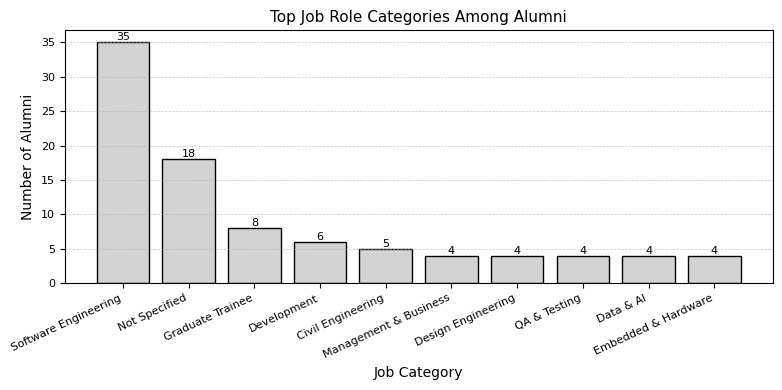
\includegraphics[width=0.7\linewidth]{figures/Chapter_3_Fig/job_distribution.png}
    \caption{Distribution of top job roles among alumni respondents}
    \label{fig:job_roles}
\end{figure}

The figure shows the distribution of job roles among 98 alumni respondents. Machine Learning Engineer has the highest representation, followed by AI Engineer and Backend Developer roles. This reflects a strong trend towards data-driven and software development careers among graduates.

\subsection{Database Schema Design}
The alumni survey data is stored using a hybrid database design approach. Core authentication and identity attributes are maintained in a normalized Users table, while alumni-specific survey responses are stored in JSON format within the Alumni table. This design provides flexibility in handling survey structures and unstructured text required for NLP-based analytics.

\section{System Architecture of EduFeedback AI}
EduFeedback AI follows a layered architecture to ensure modularity, scalability, and ease of maintenance. The system is divided into four logical layers, where each layer performs a specific function and interacts with adjacent layers.

The presentation layer provides role-based access through three interfaces: Alumni Portal, Faculty Portal, and Admin Panel. Alumni submit career details and feedback, faculty members provide course outcome attainment and academic inputs, while administrators monitor analytics and reports.

The application layer acts as the core processing unit of the system. It handles role-based logins, authentication and authorization, and exposes RESTful APIs for communication between the presentation layer and backend services.

The data analytics layer is responsible for intelligence-driven processing. It performs natural language processing using techniques such as TF-IDF and BERT, supports skill-to-curriculum mapping, calculates skill gap indices, and generates recommendations for curriculum improvement.

The data layer consists of a relational SQL database that stores alumni records, feedback data, user credentials, and analysis results. This layer ensures secure and persistent storage of all system data.

\begin{figure}[!h]
    \centering
    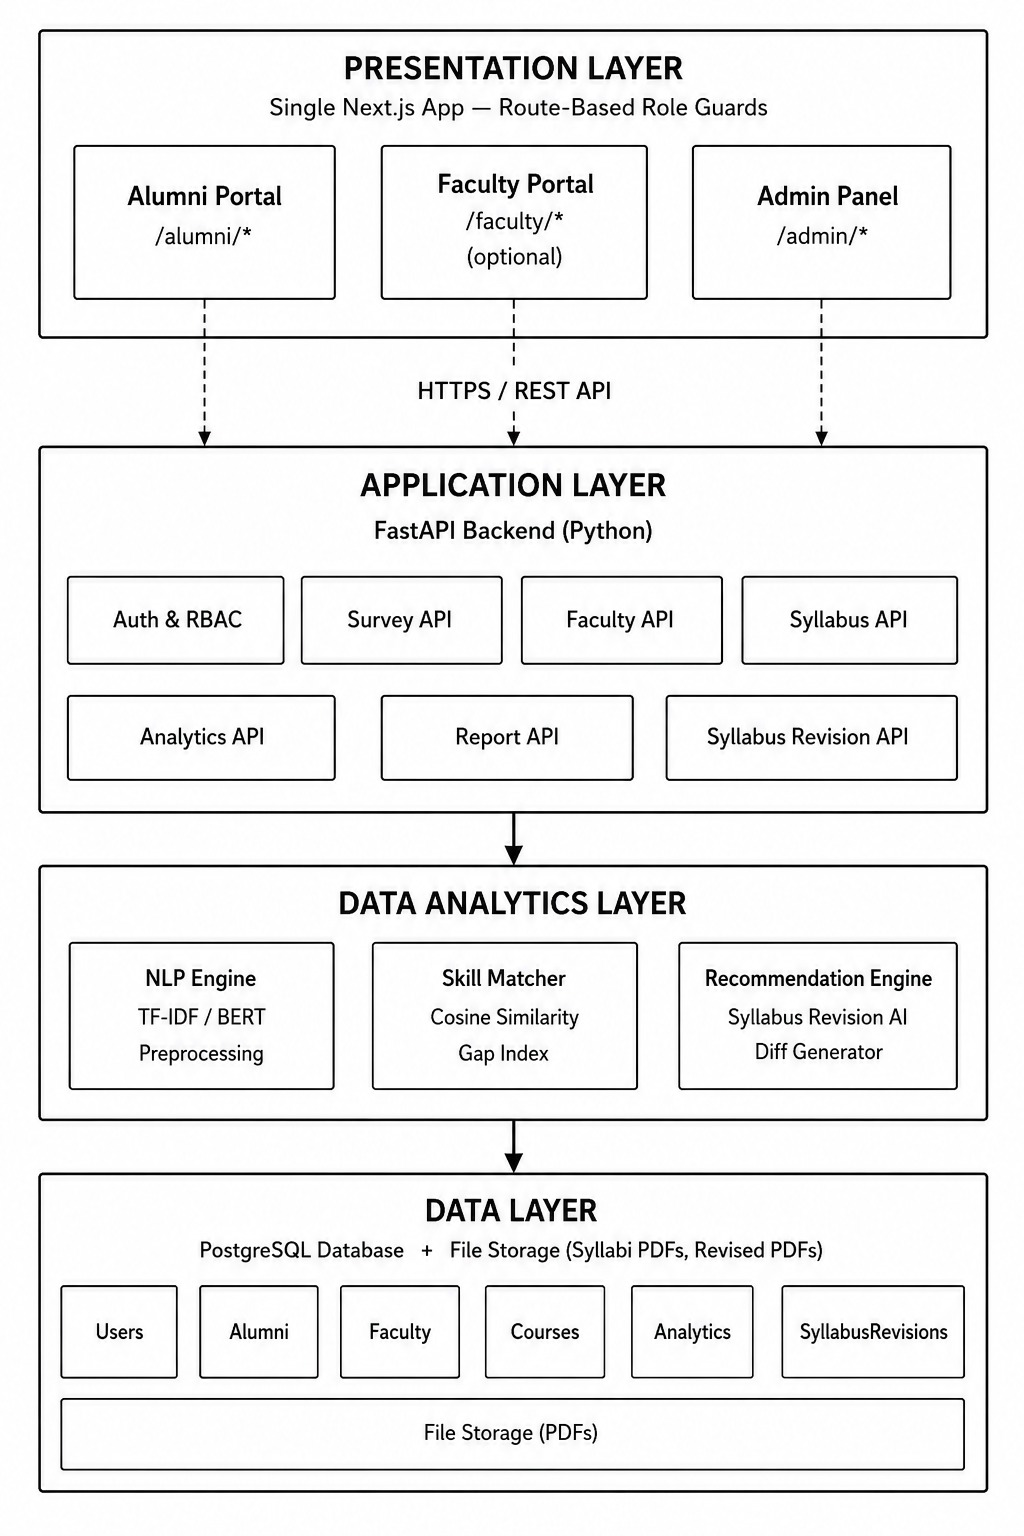
\includegraphics[width=0.7\linewidth]{figures/Chapter_3_Fig/system_architecture.png}
    \caption{System architecture of EduFeedback AI}
    \label{fig:system_architecture}
\end{figure}

\section{Identified Challenges and System Limitations}
During the planning and initial development phase, several challenges and limitations were identified:
\begin{itemize}
    \item Limited volume of alumni responses during early stages
    \item Variability in feedback quality and level of detail
    \item Difficulty in directly mapping academic subjects to diverse job roles
    \item Dependence on voluntary participation for data collection
\end{itemize}

These factors may affect the accuracy and depth of analytical results if not addressed adequately.

\section{Strategy to Address Identified Loopholes}
To mitigate the identified challenges, the following strategies are proposed:
\begin{itemize}
    \item Gradual expansion of alumni participation through structured outreach
    \item Combination of objective questions with descriptive feedback fields
    \item Standardization of skill and subject keywords to improve mapping accuracy
    \item Incremental refinement of analysis techniques as data volume increases
\end{itemize}

These measures are intended to improve data consistency, analytical reliability, and overall system effectiveness.

\section{Project Scheduling and Gantt Chart}
The project schedule is represented using a Gantt chart to illustrate the timeline and sequencing of activities across the project duration. Each phase is mapped to specific time periods, with certain tasks overlapping to ensure efficient utilization of time and timely completion of deliverables.

\begin{figure}[!htbp]
    \centering
    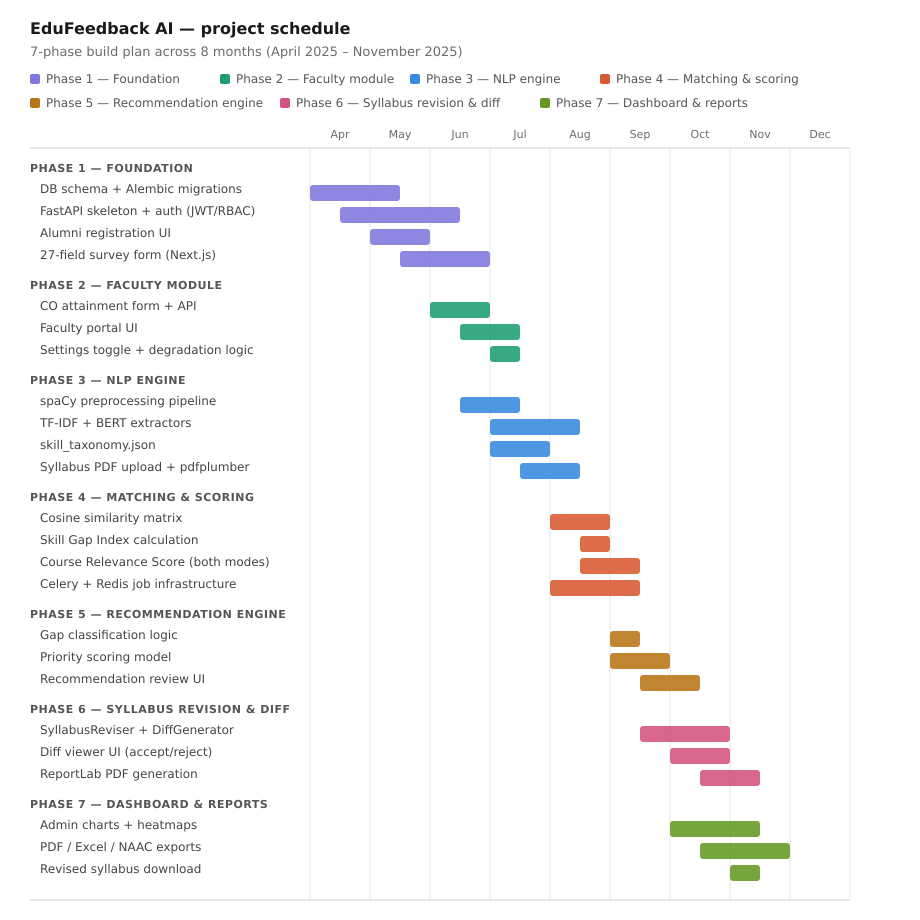
\includegraphics[width=\linewidth, height=0.85\textheight, keepaspectratio]{figures/Chapter_3_Fig/gantt_chart.png}
    \caption{Gantt chart of project schedule}
    \label{fig:gantt_chart}
\end{figure}

%% ----------------------------------------------------------------
%% Chapter_4.tex
%% ----------------------------------------------------------------
\chapter{Project Description}
\label{Chapter:Description}

\section{SOFTWARE MODEL}
EduFeedback AI follows a layered client-server architecture to make the system easier to manage, scale, and improve over time. The overall design is divided into four logical layers, with each layer handling a specific role in the system. This clear separation of responsibilities helps keep the system well-organized and reduces dependency between components. As a result, updates or improvements can be made to one part of the system without disrupting others, which supports long-term maintenance and future expansion.

The application layer is the part of the system that handles most of the working logic. It connects what the user does on the website with what happens in the backend. This layer checks who the user is, what role they have, and whether they are allowed to access a particular feature. It also makes sure that the data sent by users is valid before moving it further. When alumni submit surveys or faculty members provide course-related feedback, this layer manages how the information flows through the system. Keeping these rules in one place helps in making small changes later without affecting the full system. The data analytics layer is mainly responsible for understanding the information collected from users. Most of the feedback received is in text form and cannot be directly used for analysis. This layer processes such data and looks for useful patterns and meanings in it. It compares alumni feedback, job-related information, and course details to find how well the curriculum matches industry needs. Based on this comparison, the system highlights areas where skills are lacking and subjects that need improvement. This layer is kept flexible so that better analysis methods or new data sources can be added in the future if required.

The data analytics layer encapsulates all intelligence-driven components of the system. This layer integrates Natural Language Processing and machine learning models to analyze unstructured and semi-structured data. NLP techniques such as TF-IDF and BERT-based embeddings are employed to extract meaningful features from alumni feedback, job descriptions, and curriculum documents. Similarity computation algorithms quantify curriculum-industry alignment, while scoring models compute metrics such as the Skill Gap Index and Course Relevance Score. This layer is designed to be extensible, allowing future inclusion of advanced predictive models and external labor market datasets.

The data layer functions as the persistent storage foundation of the system. A relational database management system is used to store structured entities including user profiles, alumni career data, skill usage records, course relevance ratings, CO attainment reports, and generated analytics results. Data normalization and relational integrity constraints are enforced to ensure consistency, accuracy, and efficient query processing. This layer supports both transactional operations and analytical queries required by the dashboard and reporting components.

Overall, the layered client-server architecture enables EduFeedback AI to achieve high cohesion within modules and low coupling across layers. Such an architectural design enhances system scalability, facilitates maintenance and future upgrades, and ensures reliable performance when handling growing volumes of academic and alumni data. This design choice aligns with best practices in enterprise software development and supports the long-term adaptability of the proposed system.

\section{SOFTWARE REQUIREMENTS SPECIFICATION (SRS)}

\subsection{INTRODUCTION}
EduFeedback AI is an AI-driven academic analytics system designed to assess curriculum relevance by integrating alumni career outcomes, faculty feedback, and curriculum content. The system aims to support Outcome-Based Education (OBE) by providing quantitative and qualitative insights that assist academic administrators in curriculum evaluation and continuous improvement. This SRS document outlines the functional and non-functional requirements, system constraints, and expected performance characteristics of the proposed system.

\subsection{GENERAL DESCRIPTION}
EduFeedback AI is a web-based, client-server application developed using a layered architecture. The system supports multiple user roles, including alumni, faculty members, and administrators. Alumni provide post-graduation career data through structured surveys, faculty submit CO attainment reports, and administrators analyze aggregated insights via dashboards. The system incorporates Natural Language Processing and machine learning techniques to extract skills from unstructured text, compare them with curriculum topics, and generate curriculum refinement recommendations. The software is designed to be modular, scalable, and extensible.

\subsection{FUNCTIONAL REQUIREMENTS}
The system shall provide the following functionalities:
\begin{itemize}
    \item The system shall allow alumni to register, authenticate, and submit career outcome surveys.
    \item The system shall enable alumni to update their employment and skill-related information periodically.
    \item The system shall allow faculty members to log in and upload CO attainment reports and qualitative feedback.
    \item The system shall accept syllabus documents in text or document format for analysis.
    \item The system shall preprocess textual data using NLP techniques.
    \item The system shall extract curriculum topics and industry skills using NLP models.
    \item The system shall compute Skill Gap Index and Course Relevance Score.
    \item The system shall generate automated curriculum improvement recommendations.
    \item The system shall provide an admin dashboard with data visualization and reporting capabilities.
    \item The system shall support export of analytical reports in PDF and spreadsheet formats.
\end{itemize}

\subsection{INTERFACE REQUIREMENTS}
\textbf{User Interface}
\begin{itemize}
    \item Web-based interfaces accessible via standard browsers.
    \item Role-specific dashboards for alumni, faculty, and administrators.
    \item Responsive design to support multiple screen sizes.
\end{itemize}

\textbf{Hardware Interface}
\begin{itemize}
    \item Runs on standard desktop or laptop systems with internet connectivity.
\end{itemize}

\textbf{Software Interface}
\begin{itemize}
    \item Relational Database Management System (MySQL/PostgreSQL).
    \item NLP libraries such as scikit-learn and transformer-based models.
    \item RESTful APIs for communication between frontend and backend modules.
\end{itemize}

\subsection{PERFORMANCE REQUIREMENTS}
\begin{itemize}
    \item The system shall handle concurrent access from multiple users without degradation in performance.
    \item Response time for survey submission and dashboard queries shall not exceed acceptable web application limits.
    \item Data processing and skill-matching operations shall complete within defined time constraints for moderate data volumes.
    \item System uptime shall be maintained at a high level during academic sessions.
\end{itemize}

\subsection{DESIGN CONSTRAINTS}
\begin{itemize}
    \item The system shall be developed using open-source frameworks and tools.
    \item Data privacy and access control constraints shall be enforced.
    \item The design shall adhere to OBE, NAAC, and NBA documentation requirements.
    \item The system must be deployable on standard institutional infrastructure.
\end{itemize}

\subsection{NON-FUNCTIONAL ATTRIBUTES}
\textbf{Reliability}: The system shall ensure reliable data storage and retrieval, with safeguards against data loss.
\textbf{Security}: Role-based authentication and authorization. Secure handling of user credentials. Restricted access to sensitive academic and alumni data.
\textbf{Usability}: Simple and intuitive user interfaces. Minimal training required for users.
\textbf{Maintainability}: Modular design enables easy updates and enhancements. Clear separation between data, logic, and presentation layers.
\textbf{Scalability}: Ability to accommodate increasing numbers of users and data volume.

\section{FUNCTIONAL SPECIFICATION}

\subsection{TEXT PREPROCESSING PIPELINE}
Before features are extracted and embedded, raw textual data from alumni surveys and syllabus PDFs must be uniformly processed.

\textbf{Input Corpora}
\begin{enumerate}
    \item \textbf{Alumni Free-Text}: Extracted from survey fields (e.g., job\_responsibilities, tools\_software, skills\_acquired\_after\_graduation).
    \item \textbf{Syllabus PDF Text}: Extracted via pdfplumber (Unit headers, Learning Objectives, Topic breakdowns).
\end{enumerate}

\textbf{Processing Steps (spaCy)}
\begin{enumerate}
    \item \textbf{Lowercasing}: Convert all text to lowercase for uniformity.
    \item \textbf{Tokenization}: Split sentences into individual word tokens.
    \item \textbf{Stopword Removal}: Remove standard English stopwords and a custom academic lexicon. (e.g. {"unit", "module", "chapter", "semester", "course", "subject", "study", "learn", "understand", "basic", "introduction", "advanced"})
    \item \textbf{Lemmatization}: Reduce words to their dictionary root (e.g., "modules" $\rightarrow$ "module", "implementing" $\rightarrow$ "implement").
    \item \textbf{Entities \& N-grams}: Extract unigrams and bigrams via sliding window arrays to preserve context (e.g., "machine learning", "data structures").
\end{enumerate}

\subsection{Feature Extraction \& Embedding Models (Hybrid Ensemble)}
The system employs a Hybrid/Ensemble Feature Representation strategy for text vectorization. Rather than relying on a single traditional Machine Learning algorithm, the pipeline ensembles Statistical Keyword Scoring (TF-IDF) with Deep Contextual Embeddings (BERT). This hybrid approach ensures both rare, highly-specific technical keywords (captured by TF-IDF) and broad, conceptually similar phrases (captured by BERT) are mathematically captured.

The following Python modules and libraries strictly manage this ensemble pipeline:
\begin{itemize}
    \item \textbf{spaCy (en\_core\_web\_sm model)}: Handles linguistic rules, tokenization, and Named Entity Recognition (NER).
    \item \textbf{scikit-learn}: Powers the TF-IDF vectorization and cosine similarity matrix computations.
    \item \textbf{sentence-transformers}: Interfaces with PyTorch to provide the BERT neural network embeddings.
    \item \textbf{pdfplumber}: Handles the robust structural extraction of text and tables from legacy syllabus PDFs.
    \item \textbf{ReportLab}: Generates the finalized visually robust revised syllabus PDFs.
    \item \textbf{Celery and Redis}: Provide an asynchronous task queue to orchestrate the computationally expensive embedding processes without blocking API requests.
\end{itemize}

\textbf{TF-IDF (TERM FREQUENCY-INVERSE DOCUMENT FREQUENCY)}
Used primarily to determine the statistical importance of words across the entire institution's corpus.
\begin{itemize}
    \item Vocabulary/Max Features: 5000 (tunable).
    \item N-gram range: (1,2)
    \item Sublinear TF Scaling: Enabled to compress term frequency impact.
\end{itemize}

\textbf{BERT SEMANTIC EMBEDDINGS}
Provides deep contextual reasoning. It ensures that synonyms or distinct phrases with similar meanings map to the same vector space.
\begin{itemize}
    \item Model Selected: \texttt{sentence-transformers/all-mpnet-base-v2}
    \item Dimensionality: 768-dimensional vectors.
    \item Hardware Match: Optimized for Apple M3 Max / 36GB memory constraints without requiring heavy quantization.
\end{itemize}

\subsection{MATHEMATICAL MODEL \& SCORING FORMULA’S}
\textbf{COSINE SIMILARITY MATCHING}
The foundational operation to compare an Alumni Skill ($S$) against a Syllabus Topic ($T$) within a Course ($C$).

\[
\text{Similarity}(S, T) = \frac{E(S) \cdot E(T)}{\|E(S)\| \times \|E(T)\|}
\]

Where $E(S)$ is the BERT vector of the extracted skill, $E(T)$ is the BERT vector of the syllabus topic. Result range is [-1, 1], where values closer to 1 indicate exact semantic matches.

\textbf{SKILL GAP INDEX (SGI)}
For a specific skill $S$ reported by alumni, what is the gap in the current course $C$?
First, we find the best-matching topic in the course:
\[
\text{Best Match}(S, C) = \max_{T_i \in C} \; \text{Similarity}(S, T_i)
\]
Then, the Skill Gap Index is computed as:
\[
SGI(S, C) = 1.0 - \text{Best Match}(S, C)
\]
Note: A higher SGI indicates a wider gap.

\textbf{COURSE RELEVANCE SCORE (CRS)}
An aggregate score from 0.0 to 1.0 defining how relevant a specific course is to industry demands.
Case A: Faculty Module Enabled (CO Data Available): 
\[
CRS = (w_1 \times R_{\text{alumni}}) + (w_2 \times M_{\text{skill}}) + (w_3 \times A_{\text{CO}})
\]
Where:
\begin{itemize}
    \item $w_1, w_2, w_3$ = Institution-configured weights where $w_1 + w_2 + w_3 = 1.0$
    \item $R_{\text{alumni}}$ = Average alumni rating normalized to [0,1]
    \item $M_{\text{skill}}$ = Average cosine similarity across targeted skills mapped to the course.
    \item $A_{\text{CO}}$ = Average internal course outcome attainment percentage.
\end{itemize}

\subsection{RECOMMENDATION ENGINE LOGIC}
When a skill gap is identified, the system evaluates the importance and urgency of addressing that gap using a priority score.
\[
\text{Priority Score} = SGI \times P_{\text{mention}} \times W_{\text{recency}}
\]
Where $P_{\text{mention}}$ is Alumni Mention Percentage, and $W_{\text{recency}}$ is Recency Multiplier (1.5 if emerging trend, 1.0 otherwise).

\textbf{CLASSIFICATION RULES}
The AI flags syllabus topics applying the following deterministic thresholds:
\begin{enumerate}
    \item \textbf{Type: ADD (High Demand, Low Coverage)}
    \item \textbf{Type: REDUCE / REVIEW (Low ROI Topics)}
    \item \textbf{Type: OVERHAUL (Severe Misalignment)}
\end{enumerate}

\subsection{SYLLABUS DIFF GENERATION}
During the AI revision process, recommendations (Type ADD/REDUCE/MODIFY) need to be inserted correctly back into the syllabus structure.

\textbf{Topic Insertion Algorithm (For ADDs):} Let $R_{\text{topic}}$ be the recommended industry skill. To determine which Unit it belongs to:
\begin{enumerate}
    \item Compute cosine similarity between $E(R_{\text{topic}})$ and $E(\text{Unit\_Header}_i)$ for all units $i$ in the course.
    \item Assign the new topics to the unit where the similarity is maximized:
\[
\max_i \; \text{similarity}(R_{\text{topic}}, \text{Unit\_Header}_i)
\]
    \item If $\max(\text{similarity}) < 0.30$, propose appending a completely new unit.
\end{enumerate}

The Diff Generator then builds a JSON object marking original strings in red (REDUCE/DELETE) and proposed new strings in green (ADD), paired directly with evidence metrics ($P_{\text{mention}}$ and $W_{\text{recency}}$) to present the Diff view to the administrator.

\section{Design Specification}

\subsection{USE-CASE DIAGRAMS}

\begin{figure}[!htbp]
    \centering
    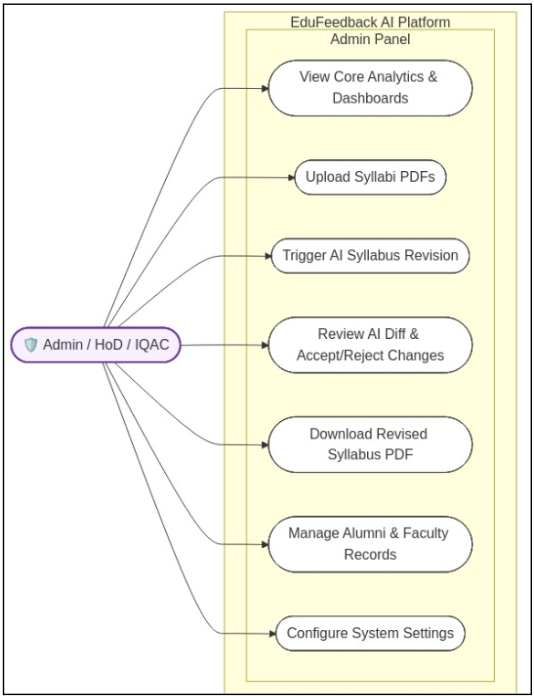
\includegraphics[width=0.65\linewidth, height=0.75\textheight, keepaspectratio]{figures/Chapter_4_Fig/uc_admin.png}
    \caption{Use-case diagram for Admin}
    \label{fig:uc_admin}
\end{figure}

\begin{figure}[!htbp]
    \centering
    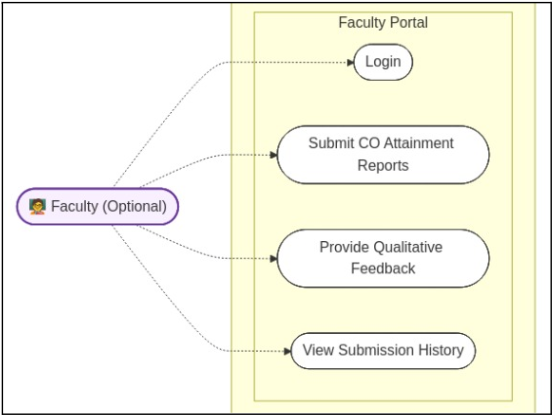
\includegraphics[width=0.65\linewidth, height=0.75\textheight, keepaspectratio]{figures/Chapter_4_Fig/uc_faculty.png}
    \caption{Use-case diagram for Faculty}
    \label{fig:uc_faculty}
\end{figure}

\begin{figure}[!htbp]
    \centering
    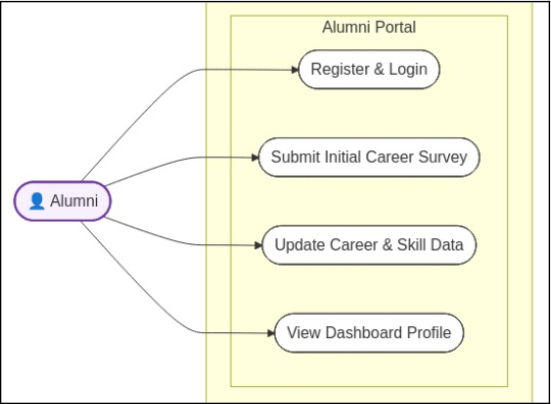
\includegraphics[width=0.65\linewidth, height=0.75\textheight, keepaspectratio]{figures/Chapter_4_Fig/uc_alumni.png}
    \caption{Use-case diagram for Alumni}
    \label{fig:uc_alumni}
\end{figure}

\clearpage
\subsection{DATA FLOW DIAGRAMS (DFD)}

\begin{figure}[!htbp]
    \centering
    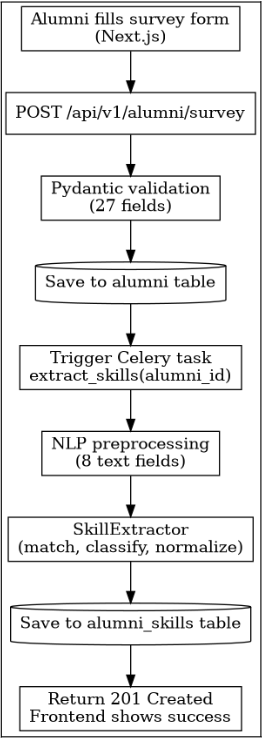
\includegraphics[width=0.75\linewidth, height=0.75\textheight, keepaspectratio]{figures/Chapter_4_Fig/dfd_alumni.png}
    \caption{Alumni Submission Flow}
    \label{fig:dfd_alumni}
\end{figure}

\begin{figure}[!htbp]
    \centering
    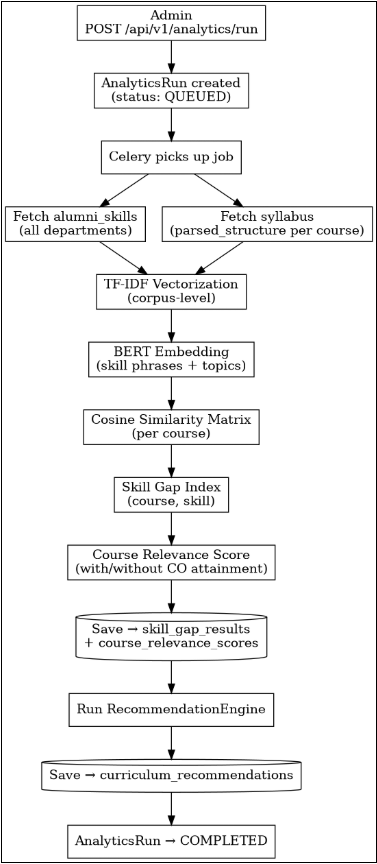
\includegraphics[width=0.75\linewidth, height=0.75\textheight, keepaspectratio]{figures/Chapter_4_Fig/dfd_nlp.png}
    \caption{NLP Analysis Flow}
    \label{fig:dfd_nlp}
\end{figure}

\begin{figure}[!htbp]
    \centering
    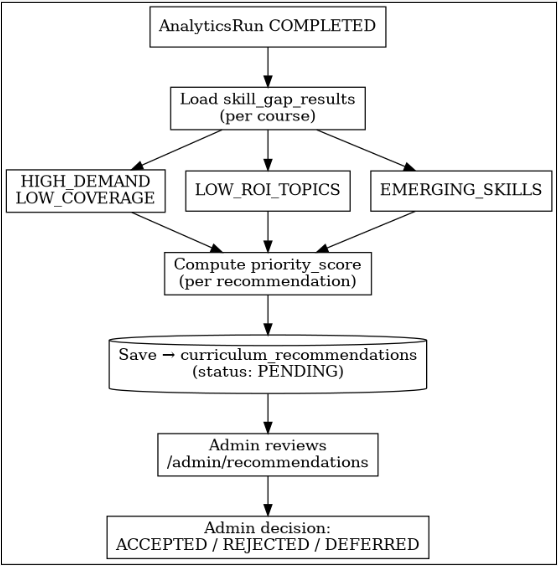
\includegraphics[width=0.75\linewidth, height=0.75\textheight, keepaspectratio]{figures/Chapter_4_Fig/dfd_recommendation.png}
    \caption{Recommendation Generation Flow}
    \label{fig:dfd_recommendation}
\end{figure}

\clearpage

\subsection{DATA DICTIONARY}

\begin{table}[h]
    \centering
    \caption{User Schema}
    \begin{tabular}{|l|l|p{5cm}|}
        \hline
        \textbf{Column} & \textbf{Type} & \textbf{Notes} \\ \hline
        id & UUID PK & \\ \hline
        email & VARCHAR UNIQUE & \\ \hline
        password\_hash & VARCHAR & bcrypt \\ \hline
        role & ENUM & alumni, faculty, admin, superadmin \\ \hline
        department\_id & FK $\rightarrow$ departments & \\ \hline
        full\_name & VARCHAR & \\ \hline
        is\_active & BOOLEAN & Default true \\ \hline
        created\_at & TIMESTAMP & \\ \hline
    \end{tabular}
\end{table}

\begin{table}[h]
    \centering
    \caption{Department Schema}
    \begin{tabular}{|l|l|p{5cm}|}
        \hline
        \textbf{Column} & \textbf{Type} & \textbf{Notes} \\ \hline
        id & UUID PK & \\ \hline
        name & VARCHAR & e.g., "Computer Science Engineering" \\ \hline
        code & VARCHAR & e.g., "CSE" \\ \hline
    \end{tabular}
\end{table}

\begin{table}[h]
    \centering
    \caption{Alumni Survey Form Schema}
    \begin{tabular}{|l|l|p{5cm}|}
        \hline
        \textbf{Column} & \textbf{Type} & \textbf{Notes} \\ \hline
        id & UUID PK & \\ \hline
        user\_id & FK $\rightarrow$ users & \\ \hline
        gender & ENUM & \\ \hline
        degree\_program & VARCHAR & \\ \hline
        department & VARCHAR & \\ \hline
        graduation\_year & INTEGER & \\ \hline
        employment\_status & ENUM & \\ \hline
        job\_role\_designation & VARCHAR & Nullable \\ \hline
        company\_name & VARCHAR & Nullable \\ \hline
        industry\_domain & VARCHAR & Nullable \\ \hline
        work\_mode & ENUM & \\ \hline
        job\_responsibilities & TEXT & NLP source; Nullable \\ \hline
        tools\_software & TEXT & NLP source; Nullable \\ \hline
        skills\_helped\_land\_job & TEXT & NLP source; Nullable \\ \hline
        course\_relevance\_rating & INTEGER & 1-5 \\ \hline
        unused\_subjects & TEXT & NLP source; Nullable \\ \hline
        skills\_missing\_from\_curriculum & TEXT & NLP source; Nullable \\ \hline
    \end{tabular}
\end{table}

\begin{table}[h]
    \centering
    \caption{Alumni Skills Schema}
    \begin{tabular}{|l|l|p{5cm}|}
        \hline
        \textbf{Column} & \textbf{Type} & \textbf{Notes} \\ \hline
        id & UUID PK & \\ \hline
        alumni\_id & FK $\rightarrow$ alumni & \\ \hline
        skill\_name & VARCHAR & Normalized form \\ \hline
        skill\_category & VARCHAR & Programming, Tool, Framework, Domain, Soft Skill \\ \hline
        source\_field & VARCHAR & Which survey field it came from \\ \hline
        is\_post\_graduation & BOOLEAN & True if from skills\_acquired\_after\_graduation \\ \hline
        extracted\_at & TIMESTAMP & \\ \hline
    \end{tabular}
\end{table}

\begin{table}[h]
    \centering
    \caption{Faculty Schema}
    \begin{tabular}{|l|l|p{5cm}|}
        \hline
        \textbf{Column} & \textbf{Type} & \textbf{Notes} \\ \hline
        id & UUID PK & \\ \hline
        user\_id & FK $\rightarrow$ users & \\ \hline
        designation & VARCHAR & \\ \hline
        specialization & VARCHAR & \\ \hline
    \end{tabular}
\end{table}

\begin{table}[h]
    \centering
    \caption{CO Attainment Reports Schema}
    \begin{tabular}{|l|l|p{5cm}|}
        \hline
        \textbf{Column} & \textbf{Type} & \textbf{Notes} \\ \hline
        id & UUID PK & \\ \hline
        faculty\_id & FK $\rightarrow$ faculty & \\ \hline
        course\_id & FK $\rightarrow$ courses & \\ \hline
        academic\_year & VARCHAR & \\ \hline
        semester & INTEGER & \\ \hline
        co\_code & VARCHAR & \\ \hline
        direct\_attainment\_pct & FLOAT & \\ \hline
        indirect\_attainment\_pct & FLOAT & \\ \hline
        final\_attainment\_pct & FLOAT & \\ \hline
        remarks & TEXT & Nullable \\ \hline
        submitted\_at & TIMESTAMP & \\ \hline
    \end{tabular}
\end{table}

\begin{table}[h]
    \centering
    \caption{Faculty Feedback Schema}
    \begin{tabular}{|l|l|p{5cm}|}
        \hline
        \textbf{Column} & \textbf{Type} & \textbf{Notes} \\ \hline
        id & UUID PK & \\ \hline
        faculty\_id & FK $\rightarrow$ faculty & \\ \hline
        course\_id & FK $\rightarrow$ courses & \\ \hline
        topics\_to\_add & TEXT & Nullable \\ \hline
        topics\_to\_remove & TEXT & Nullable \\ \hline
        student\_difficulties & TEXT & Nullable \\ \hline
        general\_comments & TEXT & Nullable \\ \hline
        submitted\_at & TIMESTAMP & \\ \hline
    \end{tabular}
\end{table}

\begin{table}[h]
    \centering
    \caption{Courses Schema}
    \begin{tabular}{|l|l|p{5cm}|}
        \hline
        \textbf{Column} & \textbf{Type} & \textbf{Notes} \\ \hline
        id & UUID PK & \\ \hline
        course\_code & VARCHAR UNIQUE & \\ \hline
        course\_name & VARCHAR & \\ \hline
        department\_id & FK $\rightarrow$ departments & \\ \hline
        semester & INTEGER & \\ \hline
        credits & INTEGER & \\ \hline
        is\_active & BOOLEAN & \\ \hline
    \end{tabular}
\end{table}

\begin{table}[h]
    \centering
    \caption{Syllabus Documents Schema}
    \begin{tabular}{|l|l|p{5cm}|}
        \hline
        \textbf{Column} & \textbf{Type} & \textbf{Notes} \\ \hline
        id & UUID PK & \\ \hline
        course\_id & FK $\rightarrow$ courses & \\ \hline
        academic\_year & VARCHAR & \\ \hline
        original\_file\_path & VARCHAR & Path to uploaded PDF \\ \hline
        parsed\_text & TEXT & Extracted plain text \\ \hline
        parsed\_structure & JSONB & Structured: units $\rightarrow$ topics $\rightarrow$ learning objectives \\ \hline
        is\_processed & BOOLEAN & Has NLP been run? \\ \hline
        uploaded\_by & FK $\rightarrow$ users & Admin who uploaded \\ \hline
        uploaded\_at & TIMESTAMP & \\ \hline
    \end{tabular}
\end{table}

\begin{table}[h]
    \centering
    \caption{Institution Settings Schema}
    \begin{tabular}{|l|l|p{5cm}|}
        \hline
        \textbf{Column} & \textbf{Type} & \textbf{Notes} \\ \hline
        id & INTEGER PK & Single row \\ \hline
        faculty\_module\_enabled & BOOLEAN & Default false \\ \hline
        relevance\_weight\_alumni & FLOAT & w1, default 0.50 \\ \hline
        relevance\_weight\_skill\_match & FLOAT & w2, default 0.50 \\ \hline
        relevance\_weight\_co\_attainment & FLOAT & w3, default 0.0 \\ \hline
        gap\_threshold & FLOAT & Min similarity to not be flagged; default 0.40 \\ \hline
        min\_alumni\_mention\_pct & FLOAT & Min \% for skill to qualify for gap analysis; default 0.10 \\ \hline
        updated\_at & TIMESTAMP & \\ \hline
    \end{tabular}
\end{table}

\begin{table}[h]
    \centering
    \caption{Skill Gap Results Schema}
    \begin{tabular}{|l|l|p{5cm}|}
        \hline
        \textbf{Column} & \textbf{Type} & \textbf{Notes} \\ \hline
        id & UUID PK & \\ \hline
        course\_id & FK $\rightarrow$ courses & \\ \hline
        skill\_name & VARCHAR & \\ \hline
        skill\_category & VARCHAR & \\ \hline
        max\_similarity\_score & FLOAT & Best cosine match vs. any syllabus topic \\ \hline
        alumni\_mention\_count & INTEGER & \\ \hline
        alumni\_mention\_pct & FLOAT & Out of total alumni \\ \hline
        is\_post\_grad\_skill & BOOLEAN & Emerged after graduation \\ \hline
        gap\_flag & BOOLEAN & True = high demand, low coverage \\ \hline
        analytics\_run\_id & FK $\rightarrow$ analytics\_runs & \\ \hline
        computed\_at & TIMESTAMP & \\ \hline
    \end{tabular}
\end{table}

\begin{table}[h]
    \centering
    \caption{Course Relevance Scores Schema}
    \begin{tabular}{|l|l|p{5cm}|}
        \hline
        \textbf{Column} & \textbf{Type} & \textbf{Notes} \\ \hline
        id & UUID PK & \\ \hline
        course\_id & FK $\rightarrow$ courses & \\ \hline
        relevance\_score & FLOAT & Final weighted composite (0-1) \\ \hline
        alumni\_relevance\_avg & FLOAT & From course\_relevance\_rating \\ \hline
        skill\_match\_score & FLOAT & From cosine similarity avg \\ \hline
        co\_attainment\_avg & FLOAT & NULL if faculty module disabled \\ \hline
        analytics\_run\_id & FK $\rightarrow$ analytics\_runs & \\ \hline
    \end{tabular}
\end{table}

\begin{table}[h]
    \centering
    \caption{Curriculum Recommendations Schema}
    \begin{tabular}{|l|l|p{5cm}|}
        \hline
        \textbf{Column} & \textbf{Type} & \textbf{Notes} \\ \hline
        id & UUID PK & \\ \hline
        course\_id & FK $\rightarrow$ courses & \\ \hline
        recommendation\_type & ENUM & ADD, REDUCE, MODIFY, REVIEW, OVERHAUL \\ \hline
        target\_topic & VARCHAR & \\ \hline
        evidence\_summary & TEXT & \\ \hline
        priority\_score & FLOAT & \\ \hline
        status & ENUM & PENDING, ACCEPTED, REJECTED, DEFERRED \\ \hline
        included\_in\_revision & BOOLEAN & Was it applied to a revised syllabus PDF? \\ \hline
        analytics\_run\_id & FK $\rightarrow$ analytics\_runs & \\ \hline
        generated\_at & TIMESTAMP & \\ \hline
    \end{tabular}
\end{table}

\begin{table}[h]
    \centering
    \caption{Syllabus Revisions Schema}
    \begin{tabular}{|l|l|p{5cm}|}
        \hline
        \textbf{Column} & \textbf{Type} & \textbf{Notes} \\ \hline
        id & UUID PK & \\ \hline
        syllabus\_document\_id & FK $\rightarrow$ syllabus\_documents & \\ \hline
        analytics\_run\_id & FK $\rightarrow$ analytics\_runs & \\ \hline
        diff\_data & JSONB & List of change objects \\ \hline
        revised\_structure & JSONB & Full revised syllabus structure \\ \hline
        revised\_pdf\_path & VARCHAR & Path to generated revised PDF; NULL until finalized \\ \hline
        applied\_changes\_count & INTEGER & \\ \hline
        rejected\_changes\_count & INTEGER & \\ \hline
        created\_by & FK $\rightarrow$ users & Admin who triggered revision \\ \hline
        finalized\_at & TIMESTAMP & When admin downloaded/finalized \\ \hline
    \end{tabular}
\end{table}

\begin{table}[h]
    \centering
    \caption{Analytics Runs Schema}
    \begin{tabular}{|l|l|p{5cm}|}
        \hline
        \textbf{Column} & \textbf{Type} & \textbf{Notes} \\ \hline
        id & UUID PK & \\ \hline
        triggered\_by & FK $\rightarrow$ users & \\ \hline
        status & ENUM & QUEUED, RUNNING, COMPLETED, FAILED \\ \hline
        started\_at & TIMESTAMP & \\ \hline
        completed\_at & TIMESTAMP & \\ \hline
        alumni\_count & INTEGER & Snapshot of data volume at run time \\ \hline
        faculty\_data\_included & BOOLEAN & Whether CO data was used in this run \\ \hline
        error\_log & TEXT & Nullable \\ \hline
    \end{tabular}
\end{table}

%% ----------------------------------------------------------------

%% ----------------------------------------------------------------
%% Chapter_5.tex
%% ----------------------------------------------------------------
\chapter{Implementation Issues}
\label{Chapter:Implementation}

The implementation of the EduFeedback AI platform involves several technical, structural, and operational complexities. While the layered system architecture provides a robust framework, the integration of distributed AI components, data processing pipelines, and user-facing interfaces introduces the following implementation challenges:

\section{Document Parsing and Data Unavailability}
A major hurdle in the pipeline is the reliable extraction of text and structural data from legacy Syllabus PDFs. Syllabi provided by various departments often lack a standardized layout, utilizing complex nested tables, multi-column formats, or even scanned images instead of digital text. While pdfplumber is utilized for text and bounding-box extraction, inconsistent document formatting leads to misclassified unit boundaries or truncated learning objectives. Ensuring the syllabus parser correctly links hierarchical topics requires robust error handling and fallback heuristics.

\section{NLP Semantic Nuances and Taxonomy Limitations}
Extracting skills accurately from alumni free-text inputs poses a challenge due to informal language, abbreviations, and overlapping terminologies. For instance, distinguishing between "Java" and "JavaScript," or mapping "Deep Learning" to an umbrella "Machine Learning" term without losing granularity required careful tuning of the skill\_taxonomy.json and spaCy NER rules. Furthermore, the Cosine Similarity calculation, while enhanced by the all-mpnet-base-v2 BERT model, occasionally suffers from high-dimensional noise when comparing highly technical sub-topics against broad academic descriptions.

\section{System Performance and Asynchronous Computing}
The computational cost of generating 768-dimensional BERT embeddings for hundreds of syllabus topics and correlating them against thousands of alumni-reported skills is intensive. Performing these operations synchronously would result in API timeouts and a degraded user experience. The implementation relies heavily on Celery and Redis to decouple these heavy workloads. Structuring the task queues to optimize memory usage (specifically managing the 36GB memory constraints of the BERT model) and avoiding database deadlocks during batched embedding writes proved to be a critical deployment issue.

\section{Cold Start Problem and Data Sparsity}
The accuracy of the Course Relevance Score and Skill Gap Index directly correlates with the volume of alumni data. During the initial phases of deployment, departments with limited alumni survey participation suffer from the "cold start" problem, where the recommendation engine lacks statistically significant evidence to flag low-ROI topics or emerging skills. The architecture gracefully degrades to rely on raw feature similarities, but the actionable intelligence is inherently constrained by the available data pool.

\section{Institutional Adoption and Subjectivity}
From an operational perspective, adjusting academic curricula mathematically using AI can face resistance from faculty members. The system was meticulously designed to keep the Faculty Module "opt-in" and to ensure the AI acts as an assistive tool (via the Diff Checker) rather than an autonomous decision-maker. Reconciling quantitative skill gaps with subjective faculty course outcome (CO) attainments requires careful weighting algorithms to prevent the AI from recommending overly radical, unaccredited changes.

%% ----------------------------------------------------------------
%% Chapter_6.tex
%% ----------------------------------------------------------------
\chapter{Conclusion, Summary and Future scope}
\label{Chapter:Conclusion}

\section{Summary of the Work}
The EduFeedback AI platform was conceptualized, architected, and modeled as an end-to-end framework to modernize academic curricula through data-driven insights. By capturing direct career outcome data from alumni—who represent the ultimate transition from academia to industry—the system algorithmically highlights the gaps between what is taught and what industry demands. The platform’s 4-tier architecture, anchored by a Next.js frontend and a FastAPI backend, seamlessly orchestrates complex data workflows. Powered by advanced Natural Language Processing (spaCy, scikit-learn, and BERT), the system transforms qualitative survey text into quantitative Skill Gap Indices and Course Relevance Scores, culminating in the automated generation of actionable, diff-mapped revised syllabus documents.

\section{Conclusion}
The traditional reliance on anecdotal feedback and manual syllabus iteration is increasingly incompatible with the rapid pace of global industry evolution. The architectural design of this system proves that integrating targeted AI matching mechanisms can effectively close this feedback loop. By generating objective, reproducible, and verifiable recommendations—while retaining administrative oversight via the Diff Checker—EduFeedback AI empowers institutional committees (such as IQAC) to make informed, highly confident decisions. The inclusion of localized reporting for bodies like NAAC and NBA directly offloads immense administrative overhead, ultimately ensuring that students are taught relevant, high-ROI skills that guarantee greater employability.

\section{Future Scope}
While the current architecture delivers a robust solution, the platform provides a strong foundational base for several advanced enhancements in the future:
\begin{itemize}
    \item \textbf{Large Language Model (LLM) Integration}: Upgrading the pipeline from BERT sentence transformers to instruction-tuned LLMs (e.g., Llama-3, GPT-4 API) could allow for more nuanced contextual reasoning, such as automatically summarizing why an emerging tool should replace an obsolete one within the Diff Checker.
    \item \textbf{Live Job Market Data Ingestion}: The system currently relies on alumni surveys. Future iterations could integrate external APIs (e.g., LinkedIn, Indeed) to continuously ingest live job descriptions, generating real-time "Industry Demand Vectors" to run parallel to alumni data.
    \item \textbf{Vision-Based Syllabus Parsing}: Integrating Vision Language Models (VLMs) could solve the complexities of parsing inconsistently formatted, legacy, or scanned PDF syllabi by intelligently processing documents as structural images rather than relying solely on raw text extraction.
    \item \textbf{Automated CO-PO Mapping Engine}: The system could be enhanced to algorithmically evaluate and update the mappings between Course Outcomes (COs) and Program Outcomes (POs) as topics are added or removed, instantly updating mandatory accreditation matrices.
    \item \textbf{Multi-Tenant SaaS Evolution}: While designed for multi-institutional capability, further refinements in isolated multi-tenant deployment, white-labeling features, and decentralized taxonomy management could transition the platform into a commercial SaaS product for widespread university adoption.
\end{itemize}


% =========================
% BACK CONTENTS OF THESIS
% =========================
\backmatter

% =========================
% BIBLIOGRAPHY
% =========================
\bibliographystyle{ieeetr}
\nocite{*}
\bibliography{bib/references}

% =========================
% APPENDIX [OPTIONAL]
% =========================
\appendix

\end{document}
%% ----------------------------------------------------------------